\section{Experimental Results}
\label{sec:experiments}

我们微调了在 ImageNet 上预训练的 VGG-16 或 ResNet-101 网络模型,以便以简单的方式按照 \cite{long2014fully} 的过程使它们适应图像语义分割任务。我们用一个分类器替换最后一层中 1000 路的 ImageNet 分类器,此分类器具有与我们语义分割任务分类一样多的目标数(包括背景)。我们的损失函数是 CNN 输出图中每个位置的交叉熵项的总和(与原始图像相比,子采样率为 8)。所有位置和标签在整体损失函数中均等加权(忽略的未标记像素除外)。目标是真实标签(子采样率为 8)。我们通过 \cite{KrizhevskyNIPS2013} 的标准 SGD 优化过程针对所有网络层的权重优化目标损失函数。假设在设置 CRF 参数时 DCNN 一元项是固定的,我们将分开训练 CNN 和 CRF。

我们在 4 个具有挑战性的数据集上评估了我们的模型:PASCAL VOC 2012、PASCAL-Context、PASCAL-Person-Part 和 Cityscapes。我们首先在 PASCAL VOC 2012 上报告了研究工作的会议版本 \cite{chen2014semantic},并推进了所有数据集上的最新结果。

\subsection{PASCAL VOC 2012}

\textbf{数据集:} PASCAL VOC 2012 分割基准 \cite{everingham2014pascal} 涉及了 20 个前景对象类和 1 个背景类。原始数据集分别包含 $1,464$ 个训练样本、$1,449$ 个验证样本和 $1,456$ 个测试样本,均已像素级标注。数据集由 \cite{hariharan2011semantic} 提供了额外的标注增益,产生了 $10,582$ 个训练样本。算法性能是由 21 个类别的平均像素交叉(IOU)来衡量的。

\subsubsection{会议版本的结果}

正如第~\ref{sec:convnet-hole}~章所述,我们在 ImageNet 上微调了 VGG-16 以适应语义分割任务。我们使用 20 张图片作为一个 mini-batch,初始学习率为 $0.001$(最终的分类器学习率为 $0.01$)。每 2000 次迭代将学习率缩小 10 倍。SGD 的动量项参数为 $0.9$,权重衰减为 $0.0005$。

DCNN 在 \textit{trainaug} 上训练完后,我们按照 \cite{krahenbuhl2011efficient} 的方式交叉验证了 CRF 模型。我们使用的缺省参数为 $w_2 = 3$ 和 $\sigma_\gamma = 3$,并通过在100张验证图片集上交叉验证搜索出了最优参数 $w_1$, $\sigma_\alpha$, $\sigma_\beta$。我们采用的是由粗到细的搜索方案。初始的搜索范围是 $w_1\in[3:6]$, $\sigma_\alpha \in [30:10:100]$, $\sigma_\beta \in [3:6]$(MATLAB 格式),然后我们根据第一轮的最优值优化搜索步长。我们进行了 10 次平均场迭代。

\begin{table}[!t]
  \centering
  \addtolength{\tabcolsep}{2.5pt}
  \scalebox{0.85}{
  \begin{tabular}{c c c | c c | c}
    \toprule[0.2em]
    {\bf Kernel} & {\bf Rate} & {\bf FOV} & {\bf Params} & {\bf Speed} & {\bf bef/aft CRF} \\
    \toprule[0.2em]
    \by{7}{7}         &    4  & 224 & 134.3M & 1.44 & 64.38 / 67.64 \\
    \by{4}{4}         &    4  & 128 & 65.1M  & 2.90 & 59.80 / 63.74 \\
    \by{4}{4}         &    8  & 224 & 65.1M  & 2.90 & 63.41 / 67.14 \\
    \by{3}{3}         &   12  & 224 & 20.5M  & 4.84 & 62.25 / 67.64 \\
    \bottomrule[0.1em]
  \end{tabular}
  }
  \caption{通过调整 `fc6' 的卷积核大小和采样率 $r$ 达到的不同效果。我们在 CRF 计算前后显示了模型的参数量、训练速度(张/秒)和验证集上的平均 IOU。DeepLab-LargeFOV(\by{3}{3}卷积核,$r=12$)达到了最佳平衡。}
  \label{tab:fov}
\end{table}


\textbf{感受野与 CRF:} 在 \tabref{tab:fov} 中,我们报告了 DeepLab 模型变体的实验,如 \secref{sec:convnet-hole} 所述这些变体使用了不同的感受野大小,通过调整 `fc6' 层中的卷积核大小与空洞采样率 $r$ 而获得。我们首先直接调整 VGG-16,使用原始的 \by{7}{7} 卷积核和 $r=4$(因为最后两个最大池化层的步长为 1)。该模型经过 CRF 后取得了 $67.64\%$ 的 IOU 性能,但是训练速度相对较慢($1.44$张/秒)。通过将卷积核大小减少到 \by{4}{4},我们将模型训练速度提高到 $2.9$ 张/秒。我们尝试了两种具有较小($r=4$)和较大($r=8$)感受野的网络变体,发现后者表现更好。最后我们决定使用大小为 \by{3}{3} 的卷积核以及更大的空洞采样率 $r=12$,通过保留 `fc6' 和 `fc7' 中 $4,096$ 个滤波器中的随机 $1,024$ 个,使得网络更加轻量。得到的模型 DeepLab-CRF-LargeFOV 与先前调整的 VGG-16(\by{7}{7}, $r=4$)性能不相上下,且 DeepLab-CRF-LargeFOV 速度更快($3.36$张/秒)、参数量更少($20.5$M而不是$134.3$M)。

CRF 大大提升了所有模型的性能,使平均 IOU 上升了 3-5\%。

\textbf{测试集评估:} 我们在 PASCAL VOC 2012 的官方测试集上评估了 DeepLab-CRF-LargeFOV 模型,达到了 $70.3\%$ 的平均 IOU。

\begin{figure*}[!htbp]
  \centering
  \scalebox{0.55} {
  \begin{tabular}{c}
    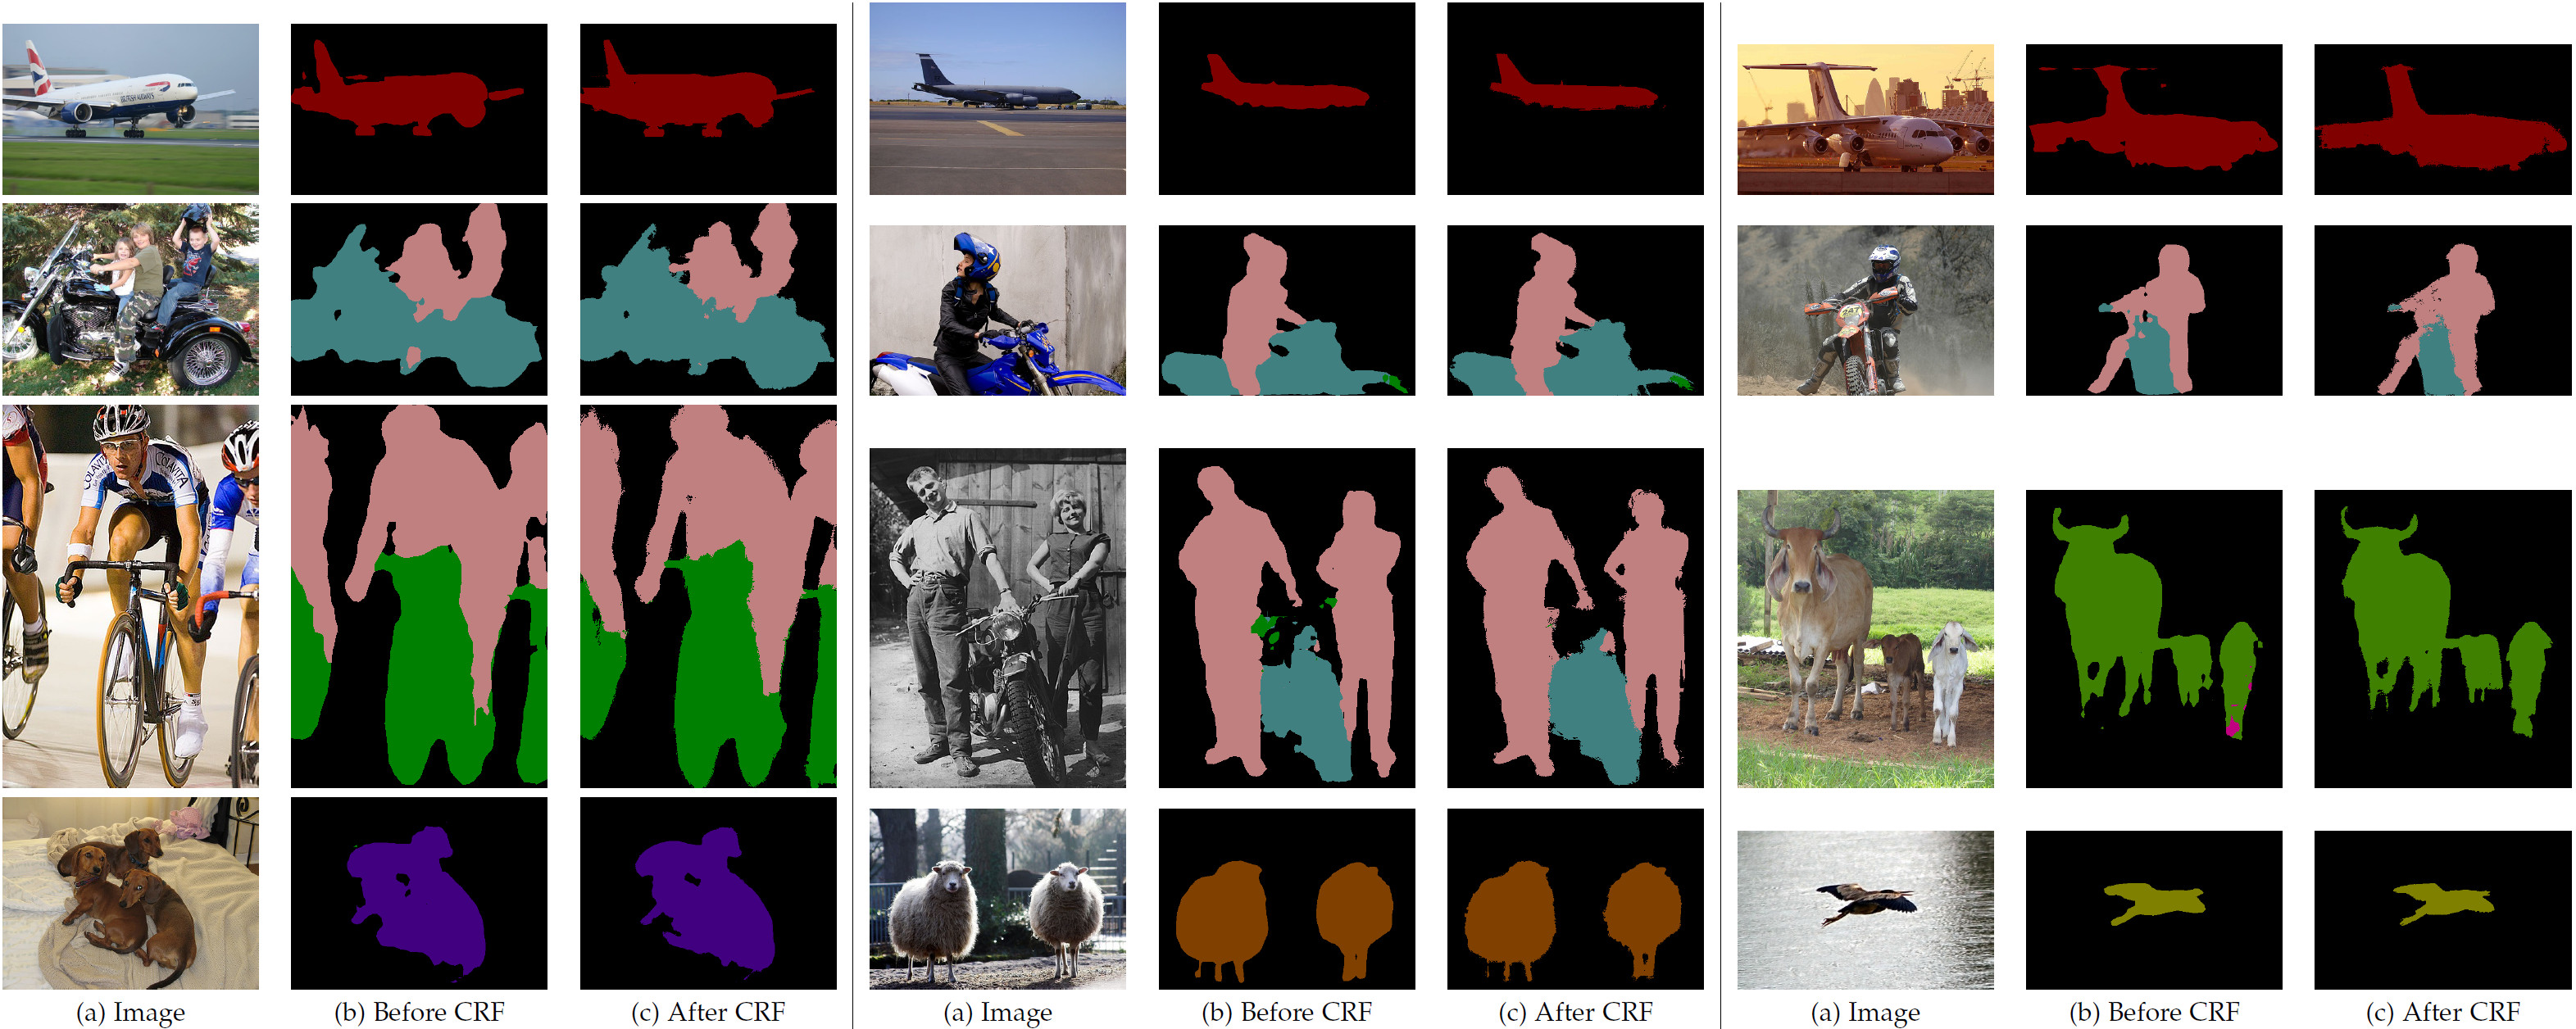
\includegraphics[width=1.8\linewidth]{fig/voc12_aspp/results.jpg}\\
  \end{tabular}
  }
  \caption{PASCAL VOC 2012 验证集结果。原始图像以及 DeepLab 处理后未经过 CRF 和 经过 CRF 的结果图像。}
  \label{fig:ValResults}
\end{figure*}


\subsubsection{会议之后的研究改进}

在这项研究工作的会议版本 \cite{chen2014semantic} 发布之后,我们对模型进行了三项主要的改进,我们将在下面讨论:(1)训练期间的不同学习策略(2)使用空洞空间金字塔池化(3)使用更深的网络结构和多尺度处理。

\textbf{学习率策略:} 在训练 DeepLab-LargeFOV 时,我们探索了不同的学习率策略。与 \cite{liu2015parsenet} 类似,我们还发现采用 ``多项式衰减'' 学习率策略(学习率乘以 $(1-\frac{iter}{max\_iter})^{power}$)比 ``分段'' 学习率(降低固定步长学习率)更有效。如 \tabref{tab:val_poly} 所示,使用 ``多项式衰减'' 策略($power=0.9$)并使用相同大小的 mini-batch 和迭代次数比 ``分段'' 策略训练出的模型在 IOU 上要高出 $1.17\%$。固定 mini-batch 大小并将训练迭代次数增加到 10K 可将 IOU 提升至 $64.90\%$(提升了 $1.48\%$);但是,由于更多的迭代次数,总训练时间增加了。然后我们将 mini-batch 大小减少到 10,发现仍然保持了相当的性能($64.90\%$ \vs $64.71\%$)。最终我们选择 mini-batch 大小为 10 以及 20 次迭代,以保证与之前 ``分段'' 策略差不多的训练时间。令人惊讶的是,这使我们在验证集上的表现为 $65.88\%$(比 ``分段'' 提高了 $3.63\%$),在测试集上表现为 $67.7\%$ (未经过 CRF)。本文中提到的所有其他实验均采用的是 ``多项式衰减'' 学习率调整策略。

\begin{table}[!t]
  \centering
  \addtolength{\tabcolsep}{2.5pt}
  \begin{tabular}{c c c c}
    \toprule[0.2 em]
    {\bf Learning policy} & {\bf Batch size} & {\bf Iteration} & {\bf mean IOU} \\
    \toprule[0.2em]
    step & 30 & 6K & 62.25 \\
    \midrule
    poly & 30 & 6K & 63.42 \\
    poly & 30 & 10K & 64.90 \\
    poly & 10 & 10K & 64.71 \\
    poly & 10 & 20K & 65.88 \\
    \bottomrule[0.1em]
  \end{tabular}
  \caption{不同超参数下模型在 PASCAL VOC 2012 验证集上的结果(\%,未经过 CRF)。训练 DeepLab-LargeFOV 时,使用 ``多项式衰减'' 比 ``分段'' 学习率更为有效。}
  \label{tab:val_poly}
\end{table}

\begin{figure}[!t]
  \centering
  \scalebox{0.85}{
  \begin{tabular}{c c}
    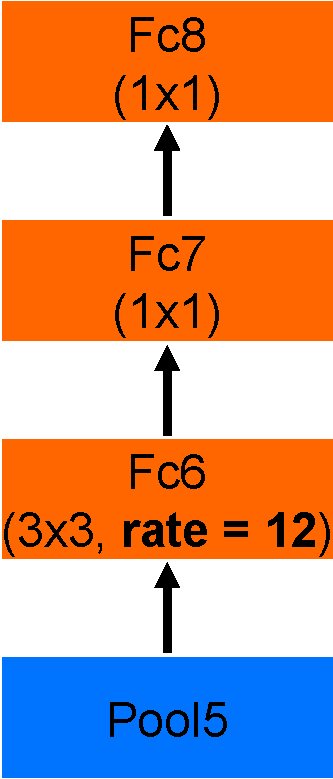
\includegraphics[width=0.2\linewidth]{./fig/spm/deeplab_largefov.pdf} &
    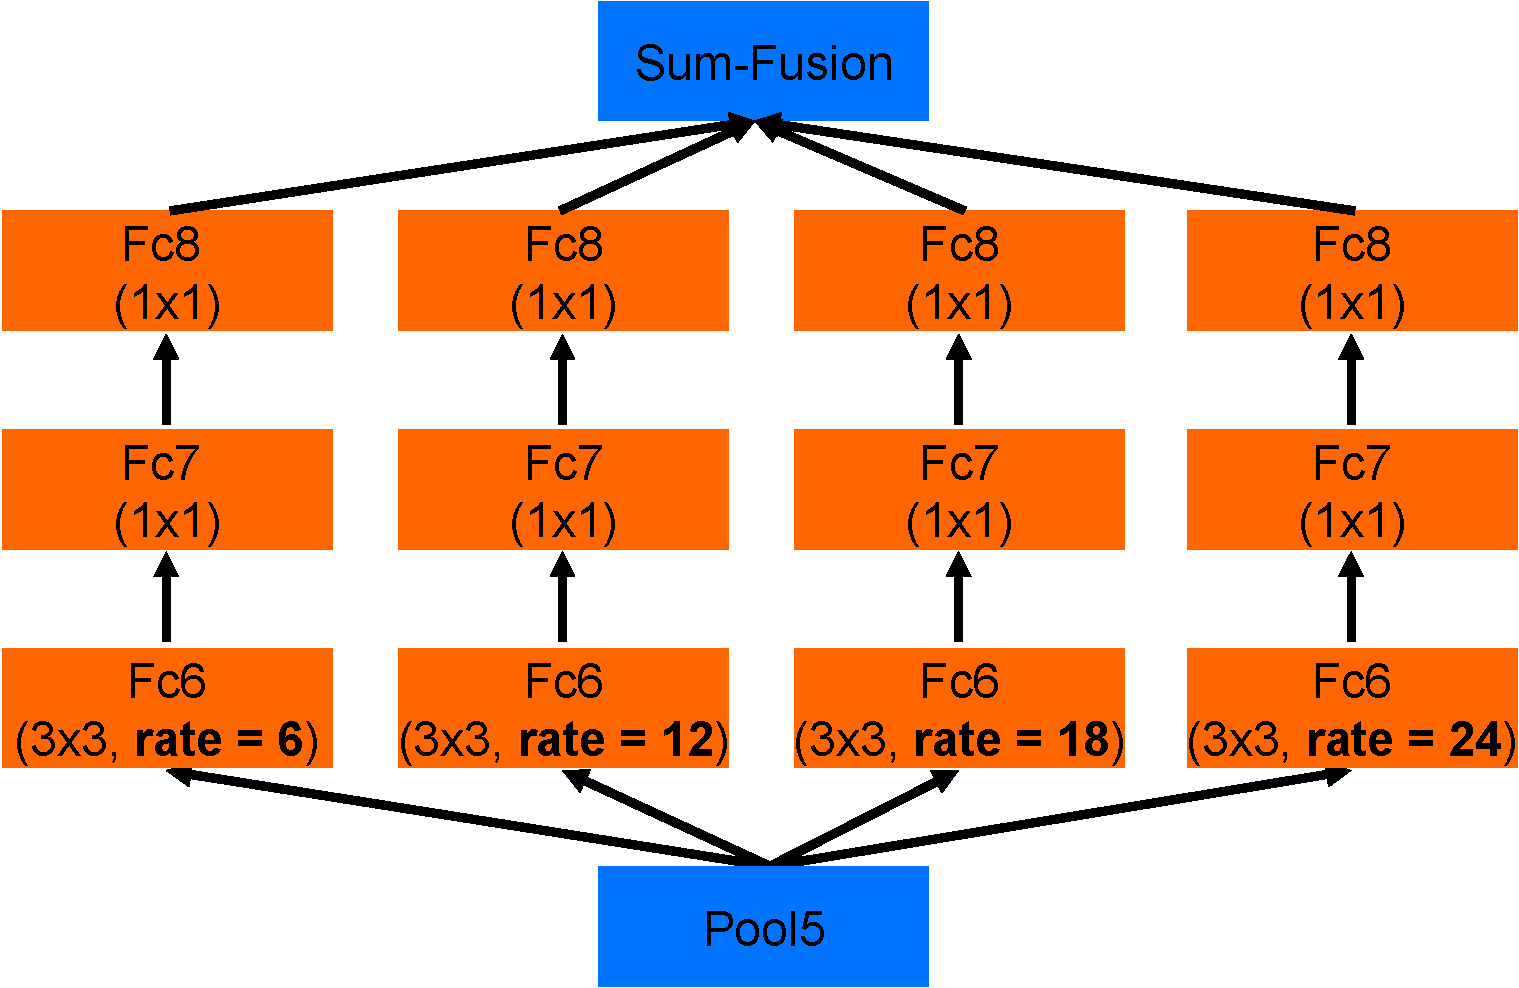
\includegraphics[height=4.5cm]{./fig/spm/deeplab_spm.pdf} \\
    {\scriptsize (a) DeepLab-LargeFOV} &
    {\scriptsize (b) DeepLab-ASPP} \\
  \end{tabular}
  }
  \caption{DeepLab-ASPP 使用多个不同采样率的滤波器来捕获不同尺度下的物体及上下文。}
  \label{fig:diff_hole}
\end{figure}

\textbf{空洞空间金字塔池化:} 我们已经尝试了 \secref{sec:convnet-hole} 中描述的 空洞空间金字塔池化(ASPP)方法。如 \figref{fig:diff_hole} 所示,VGG-16 的 ASPP 采用了几个并行的 fc6-fc7-fc8 分支。它们的 fc6 层中都使用 \by{3}{3} 大小的卷积核,但是为了捕获不同尺度的物体,它们的空洞率 $r$ 不同。在 \tabref{tab:vgg_mfov} 中,我们展示了不同设置下的结果:(1)基线 LargeFOV 模型,具有单个 $r=12$ 分支(2)ASPP-S,具有四个分支和较小的 $r=\{2,4,8,12\}$(3)ASPP-L,具有四个分支和较大的 $r=\{6,12,18,24\}$。对于每一个变体,我们记录了 CRF 前后的结果。如表中所示,在 CRF 之前,ASPP-S 比基线提高了 $1.22\%$。然而,经过 CRF 计算之后,LargeFOV 和 ASPP-S 表现差不多。另一方面,ASPP-L 在 CRF 前后均比 LargeFOV 表现要好。我们在测试集上评估了 ASPP-L + CRF 模型,达到了 $72.6\%$ 的 IOU。在 \figref{fig:aspp} 中,我们对不同的结果进行了可视化处理。

\begin{table}[!t]
  \centering
  \addtolength{\tabcolsep}{0pt}
  \begin{tabular} {c | c c }
    \toprule[0.2em]
    {\bf Method} & {\bf before CRF} & {\bf after CRF} \\
    \toprule[0.2em]
    LargeFOV & 65.76 & 69.84 \\
    ASPP-S   & 66.98 & 69.73 \\
    ASPP-L   & 68.96 & 71.57 \\
    \bottomrule[0.1em]
  \end{tabular}
  \caption{ASPP 对基于 VGG-16 的 DeepLab 模型在 PASCAL VOC 2012 验证集上的性能影响。
    {\bf LargeFOV}: 单分支, $r = 12$。
    {\bf ASPP-S}: 四分支, $r$ = \{2, 4, 8, 12\}。
    {\bf ASPP-L}: 四分支, $r$ = \{6, 12, 18, 24\}。}
  \label{tab:vgg_mfov}
\end{table}

\begin{figure}
  \centering
  \begin{tabular}{c c c c}
    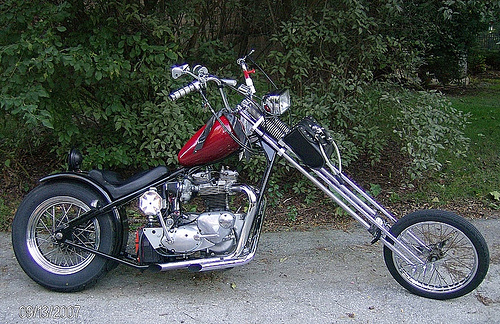
\includegraphics[width=0.21\linewidth]{fig/spm/img/2010_003947.jpg} &
    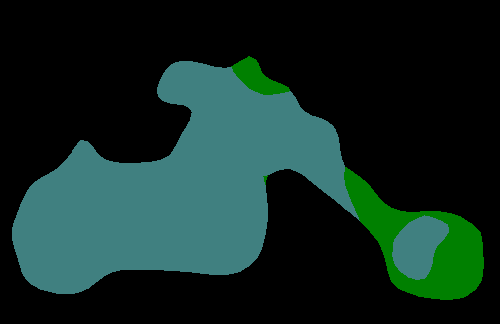
\includegraphics[width=0.21\linewidth]{fig/spm/vgg128_noup_pool3_20M_largewin3_newcode5/post_none/2010_003947.png} &
    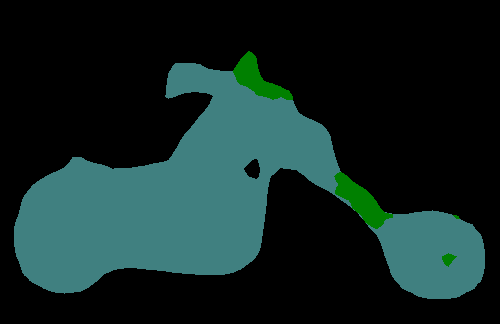
\includegraphics[width=0.21\linewidth]{fig/spm/vgg128_noup_pool3_40M_largewin_spm_2/post_none/2010_003947.png} &    
    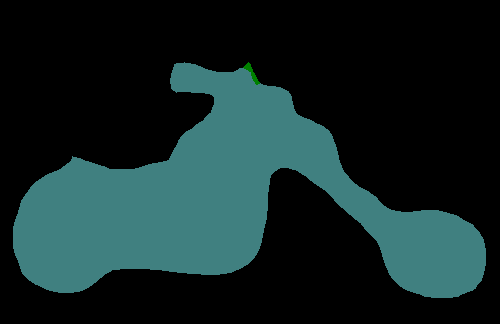
\includegraphics[width=0.21\linewidth]{fig/spm/vgg128_noup_pool3_40M_largewin_spm_3/post_none/2010_003947.png} \\
    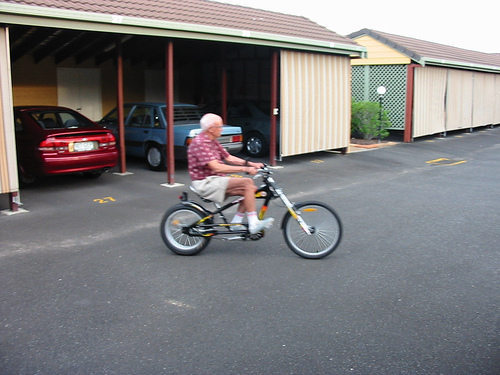
\includegraphics[width=0.21\linewidth]{fig/spm/img/2010_003446.jpg} &
    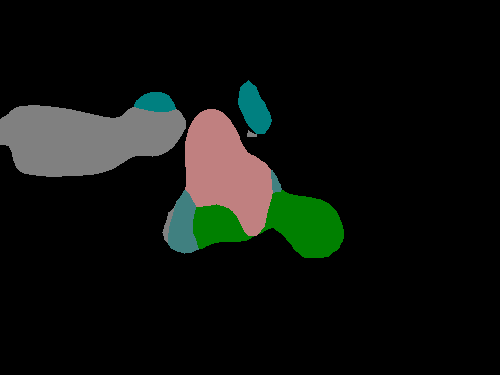
\includegraphics[width=0.21\linewidth]{fig/spm/vgg128_noup_pool3_20M_largewin3_newcode5/post_none/2010_003446.png} &
    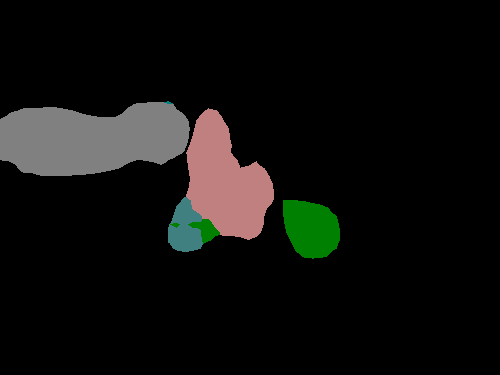
\includegraphics[width=0.21\linewidth]{fig/spm/vgg128_noup_pool3_40M_largewin_spm_2/post_none/2010_003446.png} &    
    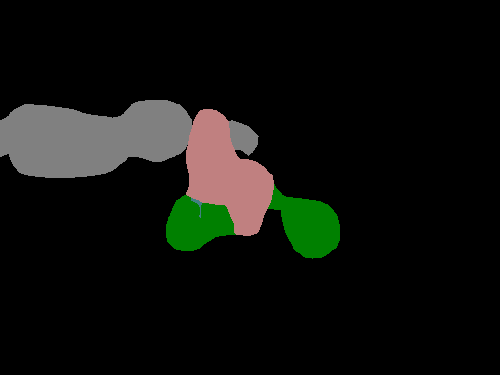
\includegraphics[width=0.21\linewidth]{fig/spm/vgg128_noup_pool3_40M_largewin_spm_3/post_none/2010_003446.png} \\
    (a) Image &
    (b) LargeFOV &
    (c) ASPP-S &
    (d) ASPP-L \\
  \end{tabular}
  \caption{与基线 LargeFOV 模型相比,ASPP 的定性分割结果。采用多个\textit{大感受野}的 \textbf{ASPP-L} 模型可以成功捕获多个尺度的物体和图像上下文。}
  \label{fig:aspp}
\end{figure}


\begin{table}[!t]
  \centering
  \addtolength{\tabcolsep}{-1pt}
  \begin{tabular} {c c c c c c | c}
    \toprule[0.2em]
    {\bf MSC} & {\bf COCO} & {\bf Aug} & {\bf LargeFOV} & {\bf ASPP} & {\bf CRF} & {\bf mIOU} \\
    \toprule[0.2em]
    & & & & & & 68.72 \\
    \checkmark & & & & & & 71.27 \\
    \checkmark & \checkmark & & & & & 73.28 \\
    \checkmark & \checkmark & \checkmark & & & & 74.87 \\
    \checkmark & \checkmark & \checkmark & \checkmark & & & 75.54 \\
    \checkmark & \checkmark & \checkmark & & \checkmark & & 76.35 \\
    \checkmark & \checkmark & \checkmark & & \checkmark & \checkmark & 77.69 \\
    \bottomrule[0.1em]
  \end{tabular}
  \caption{在 PASCAL VOC 2012 验证集上使用基于 ResNet-101 的 DeepLab。
    {\bf MSC}: 采用最大融合的多尺度输入。
    {\bf COCO}: 用 MS-COCO 数据集预训练了模型。
    {\bf Aug}: 采用随机变换输入尺度的数据增益方法。}
  \label{tab:resnet_val}
\end{table}

\textbf{更深的网络结构和多尺度处理:} 
我们已经尝试了使用最近的残差网络 ResNet-101 \cite{he2015deep} 替代 VGG-16 来构建 DeepLab。如 \secref{sec:convnet-hole} 所述,与我们对 VGG-16 网络所做的类似,我们通过空洞卷积重新使用 ResNet-101。最重要的是,我们采用了一些其他的功能,最近的研究工作有:\cite{farabet2013learning,  papandreou2015weakly, zheng2015conditional, liu2015semantic, lin2015efficient, chen2015attention, kokkinos2016pushing}(1)多尺度输入:我们分别按缩放比例 \{0.5,0.75,1\} 将图像输入给 DCNN,通过分别对每个位置的刻度进行最大响应来融合它们的得分图 \cite{chen2015attention}(2)在 MS-COCO 数据集 \cite{lin2014microsoft} 上预训练模型(3)通过在训练期间随机缩放输入图像(0.5\~1.5)来实现数据增益。在 \tabref{tab:resnet_val} 中,我们评估了每个因素以及 LargeFOV 和 ASPP 如何影响模型在验证集上的性能。我们发现,采用 ResNet-101 代替 VGG-16 显著地提高了 DeepLab 的性能(我们最简单的 ResNet-101 的模型未经过 CRF 达到了 $68.72\%$,而基于 VGG-16 的 DeepLab-LargeFOV 只有 $65.76\%$)。多尺度融合 \cite{chen2015attention} 带来了额外 $2.55\%$ 的性能提升,而在 MS-COCO 上预训练模型则获得另外 $2.01\%$ 的提升。训练期间的数据增益也是有效的(提升了 $1.6\%$)。使用 LargeFOV 也是有效的(在 ResNet-101 上添加空洞卷积层,使用 $\by{3}{3}, r=12$ 卷积核),提升了 $0.6\%$。使用空洞空间金字塔池化又将模型性能提升了 $0.8\%$。再使用全连接 CRF 对最优 DCNN 模型的结果进行再处理,达到了 $77.69\%$ 的性能。

\textbf{定性结果:} 如 \figref{fig:ValResults} 所示,我们对 CRF 前后的 DeepLab 进行了可视化处理比较。DeepLab 在 CRF 之前就产生了出色的分割结果,使用 CRF 后消除了误报且细化了物体边界,进一步提升了性能。

\textbf{测试集结果:} 我们将最终最佳模型的结果提交给数据集官方服务器,如 \tabref{tab:res_testset} 所示,官方反馈了 $79.7\%$ 的测试集性能。该模型大大优于以前的 DeepLab 变体(比如基于 VGG-16 的 DeepLab-LargeFOV),并且在 PASCAL VOC 2012 语义分割任务上一举夺魁。

\begin{table}[!th]
  \centering
  \addtolength{\tabcolsep}{2.5pt}
  \begin{tabular}{l | c}
    \toprule[0.2 em]
    {\bf Method} & {\bf mIOU} \\
    \toprule[0.2 em]
    DeepLab-CRF-LargeFOV-COCO \cite{papandreou2015weakly} & 72.7\\
    MERL\_DEEP\_GCRF \cite{Vemulapalli2016Gaussian} & 73.2 \\
    CRF-RNN \cite{zheng2015conditional} & 74.7 \\
    POSTECH\_DeconvNet\_CRF\_VOC \cite{noh2015learning} & 74.8 \\
    BoxSup \cite{dai2015boxsup} & 75.2 \\
    Context + CRF-RNN \cite{yu2015multi} & 75.3 \\
    $QO_4^{mres}$ \cite{chandra2016fast} & 75.5 \\
    DeepLab-CRF-Attention \cite{chen2015attention} & 75.7 \\
    CentraleSuperBoundaries++ \cite{kokkinos2016pushing} & 76.0 \\
    DeepLab-CRF-Attention-DT  \cite{chen2015semantic} & 76.3 \\
    H-ReNet + DenseCRF \cite{yan2016combining} & 76.8 \\
    LRR\_4x\_COCO \cite{ghiasi2016laplacian} & 76.8 \\
    DPN \cite{liu2015semantic} & 77.5 \\
    Adelaide\_Context \cite{lin2015efficient} & 77.8 \\
    Oxford\_TVG\_HO\_CRF \cite{arnab2015higher} & 77.9 \\
    Context CRF + Guidance CRF \cite{Shen2016Fast} & 78.1 \\
    Adelaide\_VeryDeep\_FCN\_VOC \cite{wu2016bridging} & 79.1 \\
    \midrule
    \href{http://host.robots.ox.ac.uk:8080/anonymous/FLHY8R.html}{DeepLab-CRF (ResNet-101)} & 79.7 \\
    \bottomrule[0.1 em]
  \end{tabular}
  \caption{在 PASCAL VOC 2012 测试集上表现出的性能。我们在官方排行榜结果之上添加了最近 arXiv 论文的一些结果。}
  \label{tab:res_testset}
\end{table}

\textbf{VGG-16 \vs ResNet-101:}
我们发现,如 \figref{fig:res_vs_vgg_results} 所示,基于 ResNet-101 \cite{he2015deep} 的 DeepLab 比基于 VGG-16 的在物体边界上有着更好的分割结果。我们认为 ResNet-101 的特性映射 \cite{he2016identity} 具有与超列功能 \cite{hariharan2014hypercolumns} 类似的效果,它利用中间层的功能来更好地定位边界。如 \figref{fig:IOUBoundary} 所示,我们使用 ``trimap'' \cite{kohli2009robust, krahenbuhl2011efficient}(沿着物体边界的一个窄带)进一步量化了这个结果。如图所示,在CRF之前使用ResNet-101在物体边界上具有与将VGG-16与CRF结合使用时几乎相同的精度。 使用CRF对ResNet-101结果进行后处理可进一步改善分割结果。

\begin{figure}[!t]
  \centering
  \scalebox{0.85} {
  \begin{tabular}{c @{\hskip 5pt} c @{\hskip 5pt} c @{\hskip 5pt} c @{\hskip 5pt} c}

    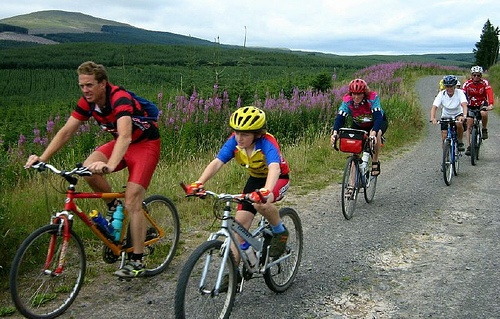
\includegraphics[width=0.21\linewidth]{fig/res_vs_vgg/resnet101_noup_pool3_14/img/2007_001311.jpg} &
    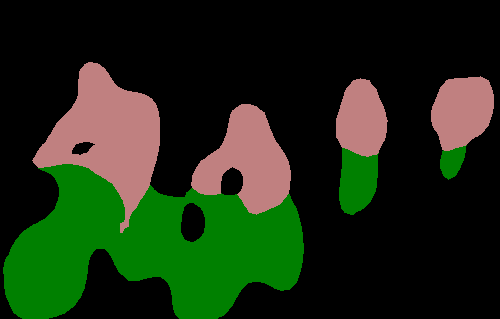
\includegraphics[width=0.21\linewidth]{fig/res_vs_vgg/vgg128_noup_pool3_20M_largewin3_newcode5/res_none/2007_001311.png} &
    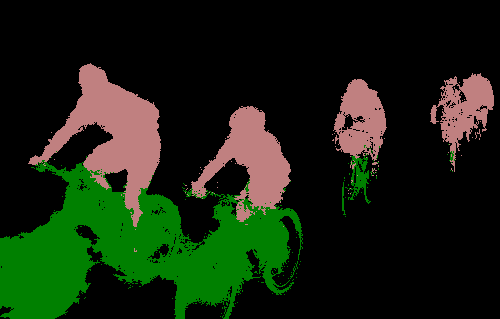
\includegraphics[width=0.21\linewidth]{fig/res_vs_vgg/vgg128_noup_pool3_20M_largewin3_newcode5/res_crf/2007_001311.png} &
    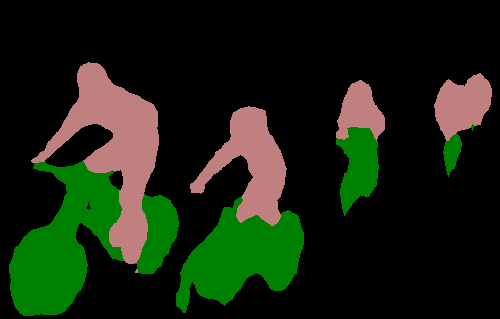
\includegraphics[width=0.21\linewidth]{fig/res_vs_vgg/resnet101_noup_pool3_14/res_none/2007_001311.png} &
    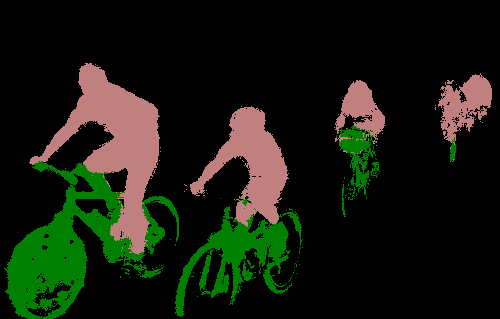
\includegraphics[width=0.21\linewidth]{fig/res_vs_vgg/resnet101_noup_pool3_14/res_crf/2007_001311.png} \\

    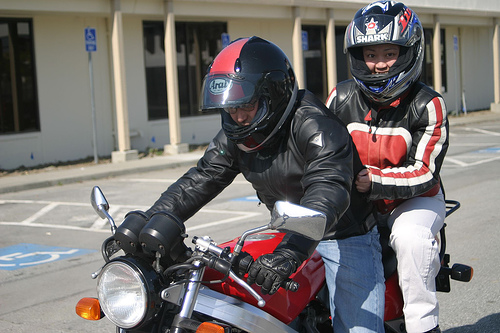
\includegraphics[width=0.21\linewidth]{fig/res_vs_vgg/resnet101_noup_pool3_14/img/2011_000455.jpg} &
    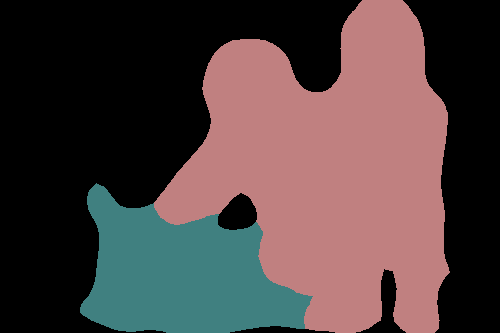
\includegraphics[width=0.21\linewidth]{fig/res_vs_vgg/vgg128_noup_pool3_20M_largewin3_newcode5/res_none/2011_000455.png} &
    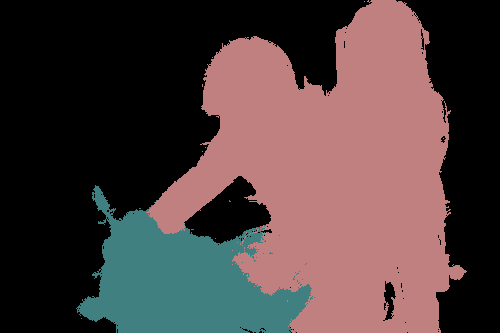
\includegraphics[width=0.21\linewidth]{fig/res_vs_vgg/vgg128_noup_pool3_20M_largewin3_newcode5/res_crf/2011_000455.png} &
    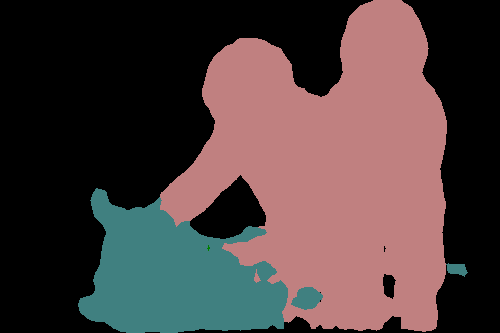
\includegraphics[width=0.21\linewidth]{fig/res_vs_vgg/resnet101_noup_pool3_14/res_none/2011_000455.png} &
    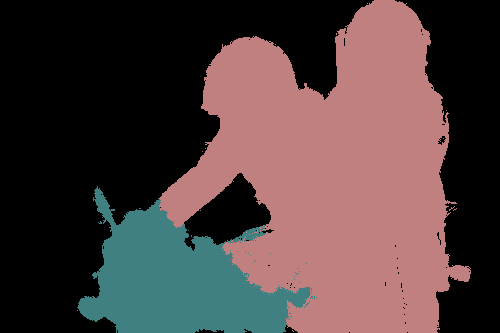
\includegraphics[width=0.21\linewidth]{fig/res_vs_vgg/resnet101_noup_pool3_14/res_crf/2011_000455.png} \\

    {\scriptsize Image} &
    {\scriptsize VGG-16 Bef.} &
    {\scriptsize VGG-16 Aft.} &
    {\scriptsize ResNet Bef.} &
    {\scriptsize ResNet Aft.} \\
  \end{tabular}
  }
  \caption{基于 ResNet-101 与 VGG-16 的 DeepLab 在 CRF 前后的结果。CRF 对于使用 VGG-16 的模型沿物体边界进行精确预测至关重要,而ResNet-101甚至在CRF之前就具有不错性能。}
  \label{fig:res_vs_vgg_results}
\end{figure}

\begin{figure}[!t]
\centering
\resizebox{\columnwidth}{!}{
  \begin{tabular} {c c}
    \raisebox{1cm} {
    \begin{tabular}{c c}
      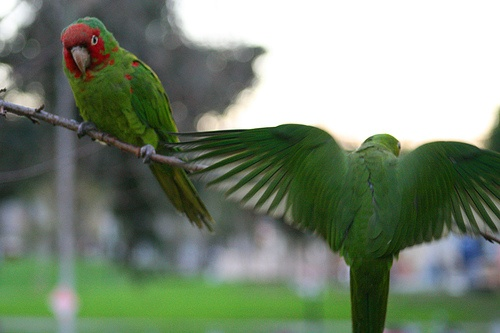
\includegraphics[height=0.1\linewidth]{fig/trimap/2007_000363.jpg} &
      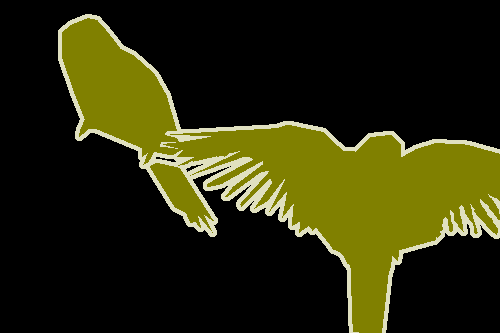
\includegraphics[height=0.1\linewidth]{fig/trimap/2007_000363.png} \\
      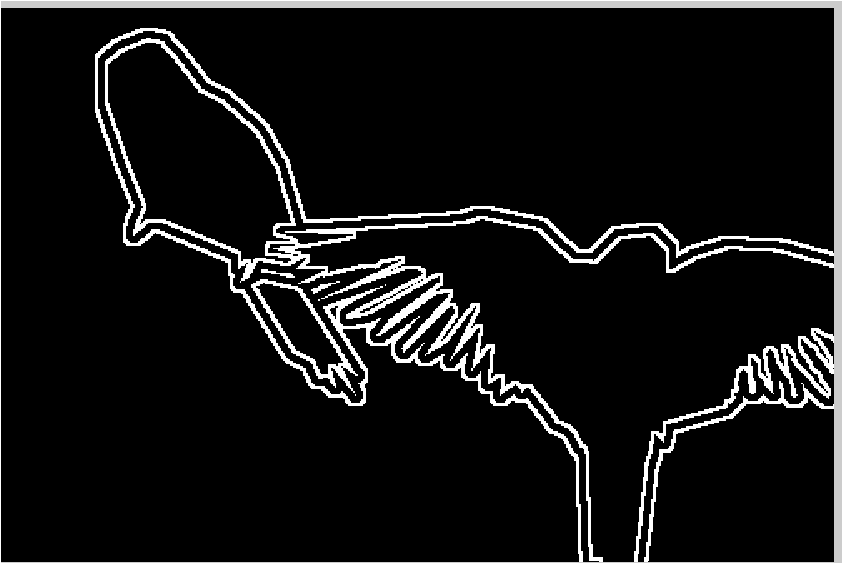
\includegraphics[height=0.1\linewidth]{fig/trimap/TrimapWidth2.pdf} &
      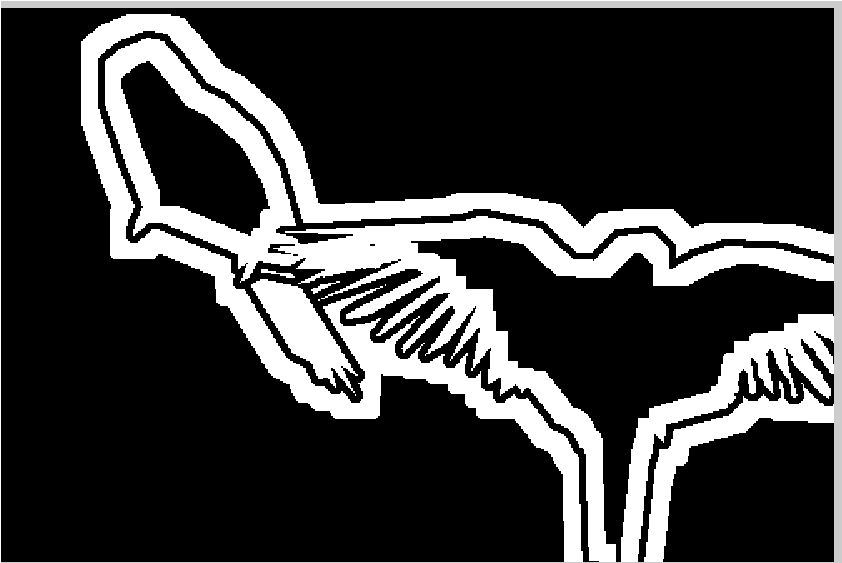
\includegraphics[height=0.1\linewidth]{fig/trimap/TrimapWidth10.pdf} \\
    \end{tabular} } &
    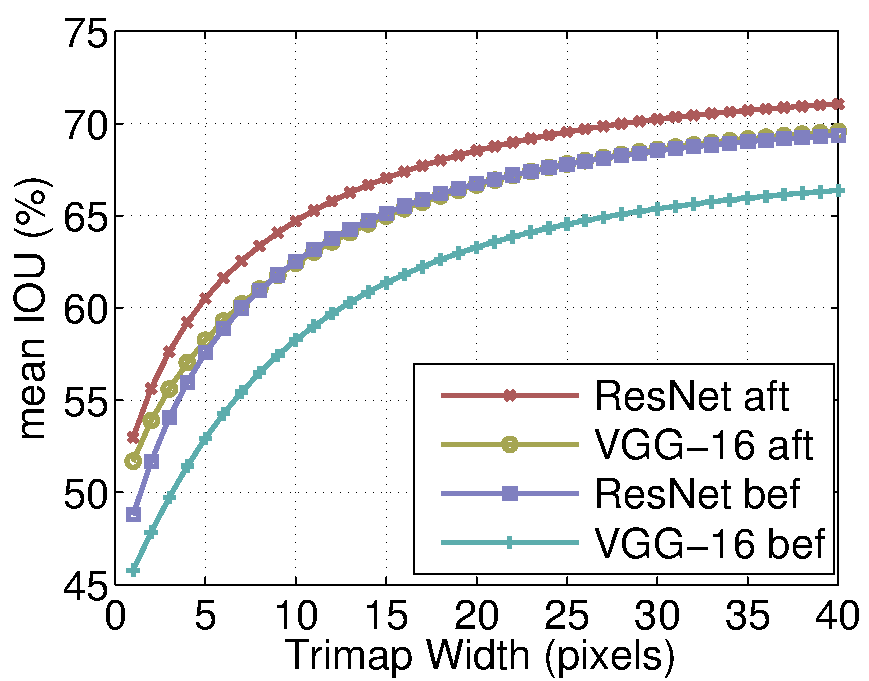
\includegraphics[height=0.25\linewidth]{fig/res_vs_vgg/SegPixelIOUWithinTrimap_ResVsVGG} \\
    (a) & (b) \\
   \end{tabular}
}
  \caption{(a)Trimap 结果 (左上: 原图。 右上: 真实边界。左下:2像素大小的 trimap。右下: 10像素大小的 trimap)。(b) 使用 VGG-16 与 ResNet-101 在 CRF 前后 的 mIOU-Trimap宽度函数曲线变化图。}
  \label{fig:IOUBoundary}
\end{figure}


\subsection{PASCAL-Context}
\label{exp:pascal_context}

\begin{figure*}[!t]
  \centering
  \scalebox{0.9} {
  \begin{tabular}{c}
    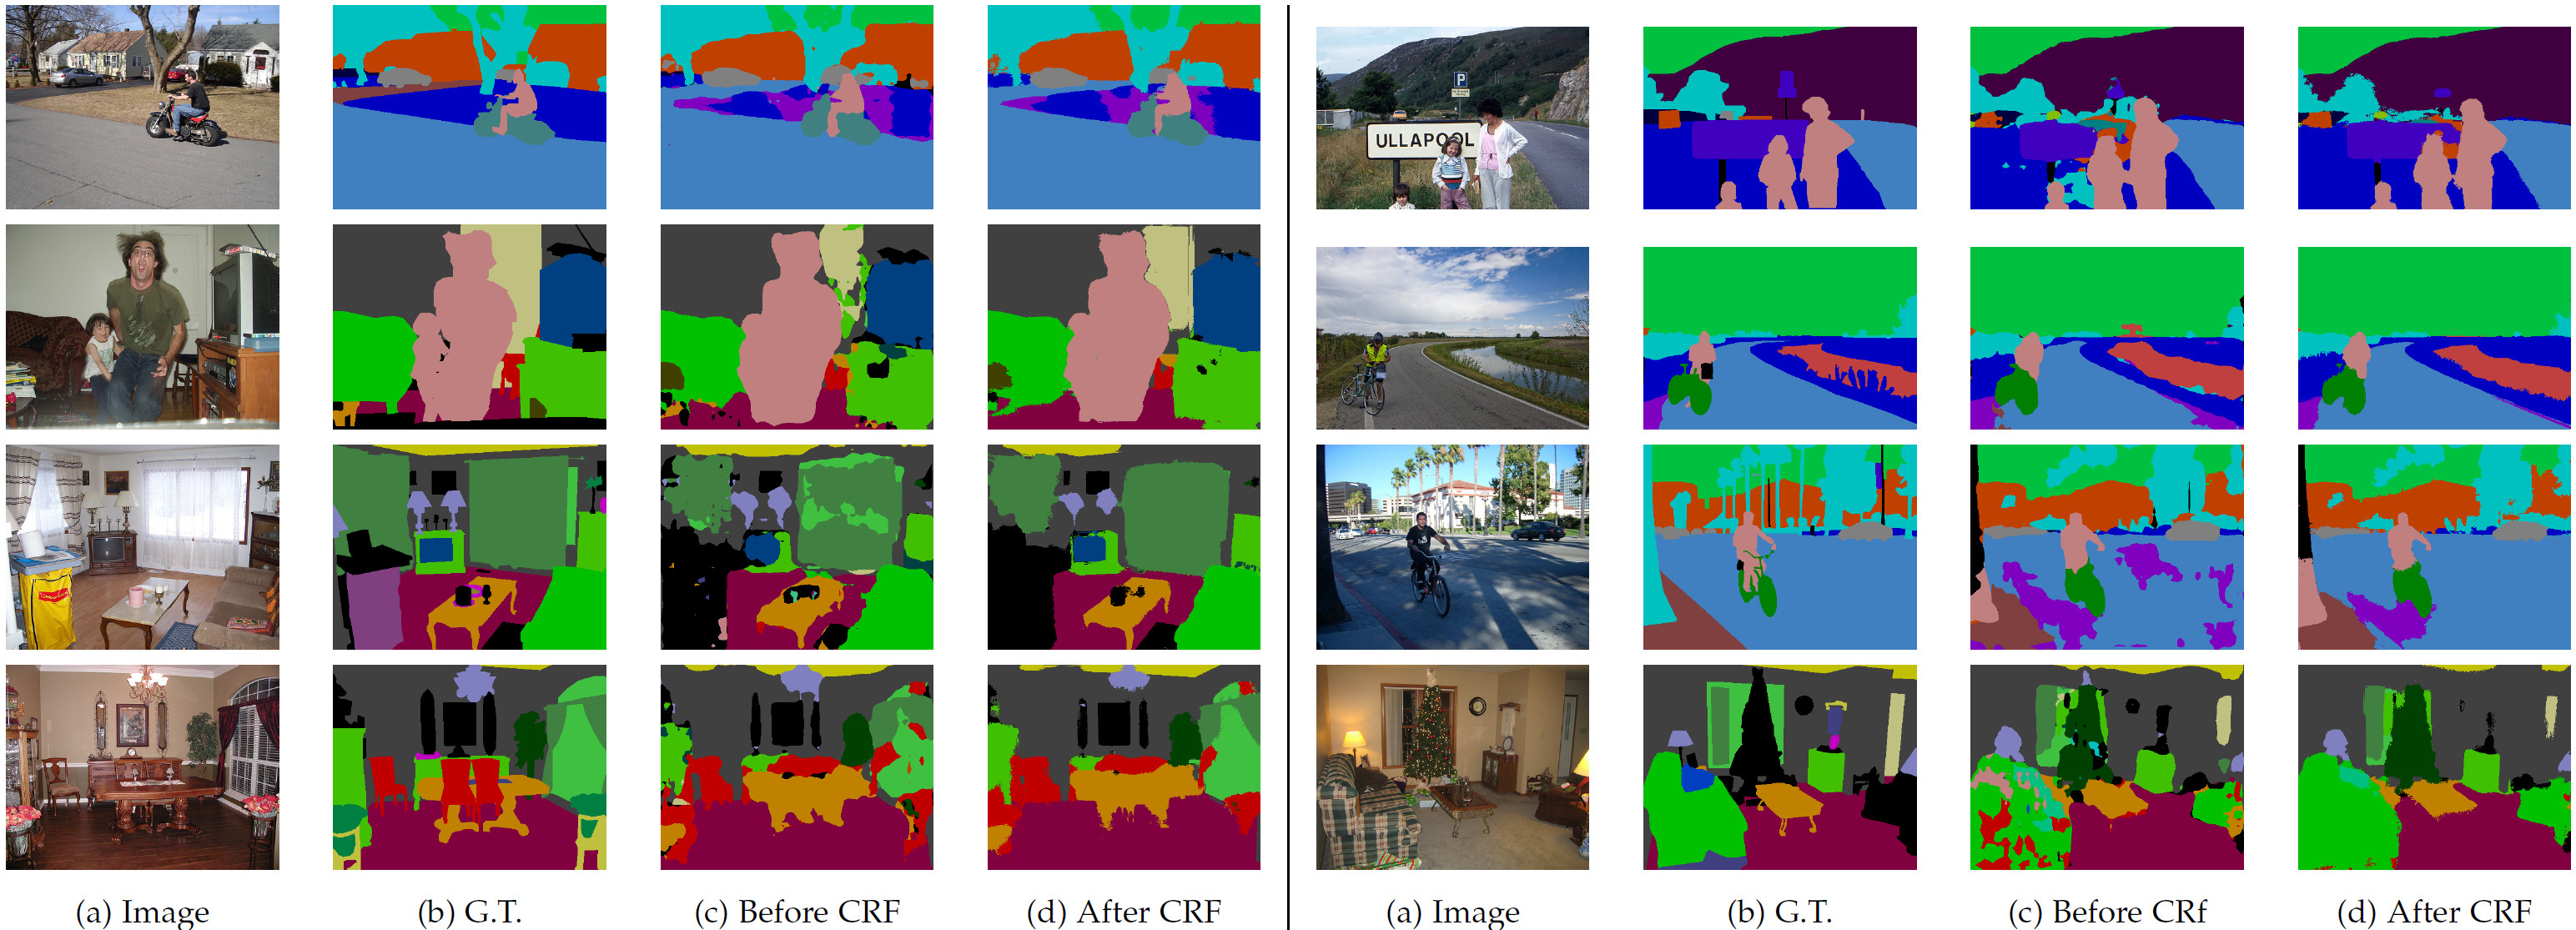
\includegraphics[width=1\linewidth]{fig/pascal_context/results.jpg} \\
  \end{tabular}
  }
  \caption{PASCAL-Context 结果。原图,真实边界,CRF前后 DeepLab 的运算结果。}
  \label{fig:pascal_context_val_results}
\end{figure*}

\begin{table}[!t]
  \centering
  \addtolength{\tabcolsep}{-3pt}
  \begin{tabular} {l c c c c c c | c}
    \toprule[0.2 em]
    {\bf Method} & {\bf MSC} & {\bf COCO} & {\bf Aug} & {\bf LargeFOV} & {\bf ASPP} & {\bf CRF} & {\bf mIOU} \\
    \toprule[0.2 em]
    \multicolumn{7}{l}{\it VGG-16} & \\
    DeepLab \cite{chen2014semantic}& & & &\checkmark & & & 37.6 \\
    DeepLab \cite{chen2014semantic}& & & &\checkmark & & \checkmark  &  39.6 \\
    \midrule
    \multicolumn{7}{l}{\it ResNet-101} & \\
    DeepLab & & & & & & &  39.6 \\
    DeepLab &\checkmark & & \checkmark & & & &  41.4 \\
    DeepLab &\checkmark &\checkmark & \checkmark & & & &  42.9 \\
    DeepLab &\checkmark &\checkmark & \checkmark & \checkmark & & & 43.5 \\
    DeepLab &\checkmark &\checkmark & \checkmark & & \checkmark & & 44.7 \\
    DeepLab &\checkmark &\checkmark & \checkmark & & \checkmark & \checkmark & 45.7 \\
    \midrule \midrule
    $O_2P$ \cite{carreira2012semantic}& & & & & &  & 18.1 \\
    CFM \cite{dai2014convolutional}& & & & & &  & 34.4 \\
    FCN-8s \cite{long2014fully}& & & & & &  & 37.8 \\
    CRF-RNN \cite{zheng2015conditional}& & & & & &  & 39.3 \\
    ParseNet \cite{liu2015parsenet}& & & & & &  & 40.4 \\
    BoxSup \cite{dai2015boxsup}& & & & & &  & 40.5 \\
    HO\_CRF \cite{arnab2015higher}& & & & & &  & 41.3 \\
    Context \cite{lin2015efficient}& & & & & &  & 43.3 \\
    VeryDeep \cite{wu2016bridging}& & & & & &  & 44.5 \\
    \bottomrule[0.1 em]
  \end{tabular}
  \caption{与 PASCAL-Context 数据集上其它优质算法的比较。}
  \label{tab:pascal_context}
\end{table}

\textbf{数据集:}
PASCAL-Context 数据集 \cite{mottaghi2014role} 为整个场景提供了详细的语义标注,包括物体(\eg, 人)和背景(\eg, 天空)。根据 \cite{mottaghi2014role},我们的模型在最常见的 59 个类别和一个背景类别上进行评估。训练集和验证集包含 $4,998$ 和 $5,105$ 张图片。

\textbf{评估:} 
我们在 \tabref{fig:pascal_context_val_results} 上显示了评估结果。基于 VGG-16 的 LargeFOV 变体在 CRF 前后的 IOU 为 $37.6\%$ 与 $39.6\%$。基于 ResNet-101 \cite{he2015deep} 的 LargeFOV 变体比 VGG-16 版本提升了 $2\%$。与 \cite{chen2015attention} 类似,使用多尺度输入和最大池化合并结果可将性能提升至 $41.4\%$。在 MS-COCO 上预训练模型可带来额外 $1.5\%$ 的性能提升。使用空洞空间金字塔池化 比 LargeFOV 更为有效。在进一步使用全连接 CRF 后,最终我们的模型达到了 $45.7\%$,比之前最好的方法 \cite{lin2015efficient} 要高 $2.4\%$,且我们未使用他们提出的非线性成对项。我们的模型也略优于 \cite{wu2016bridging},它也使用了空洞卷积来调整 \cite{he2015deep} 的残差网络进行语义分割。

\textbf{定性结果:} 如 \figref{fig:pascal_context_val_results} 所示,我们对 CRF 前后的 DeepLab 进行了可视化处理比较。DeepLab 在 CRF 之前就产生了出色的分割结果,使用 CRF 后消除了误报且细化了物体边界,进一步提升了性能。

\subsection{PASCAL-Person-Part}
\label{exp:pascal_person_part}

\begin{figure*}[!th]
  \centering
  \scalebox{0.9} {
  \begin{tabular}{c}
    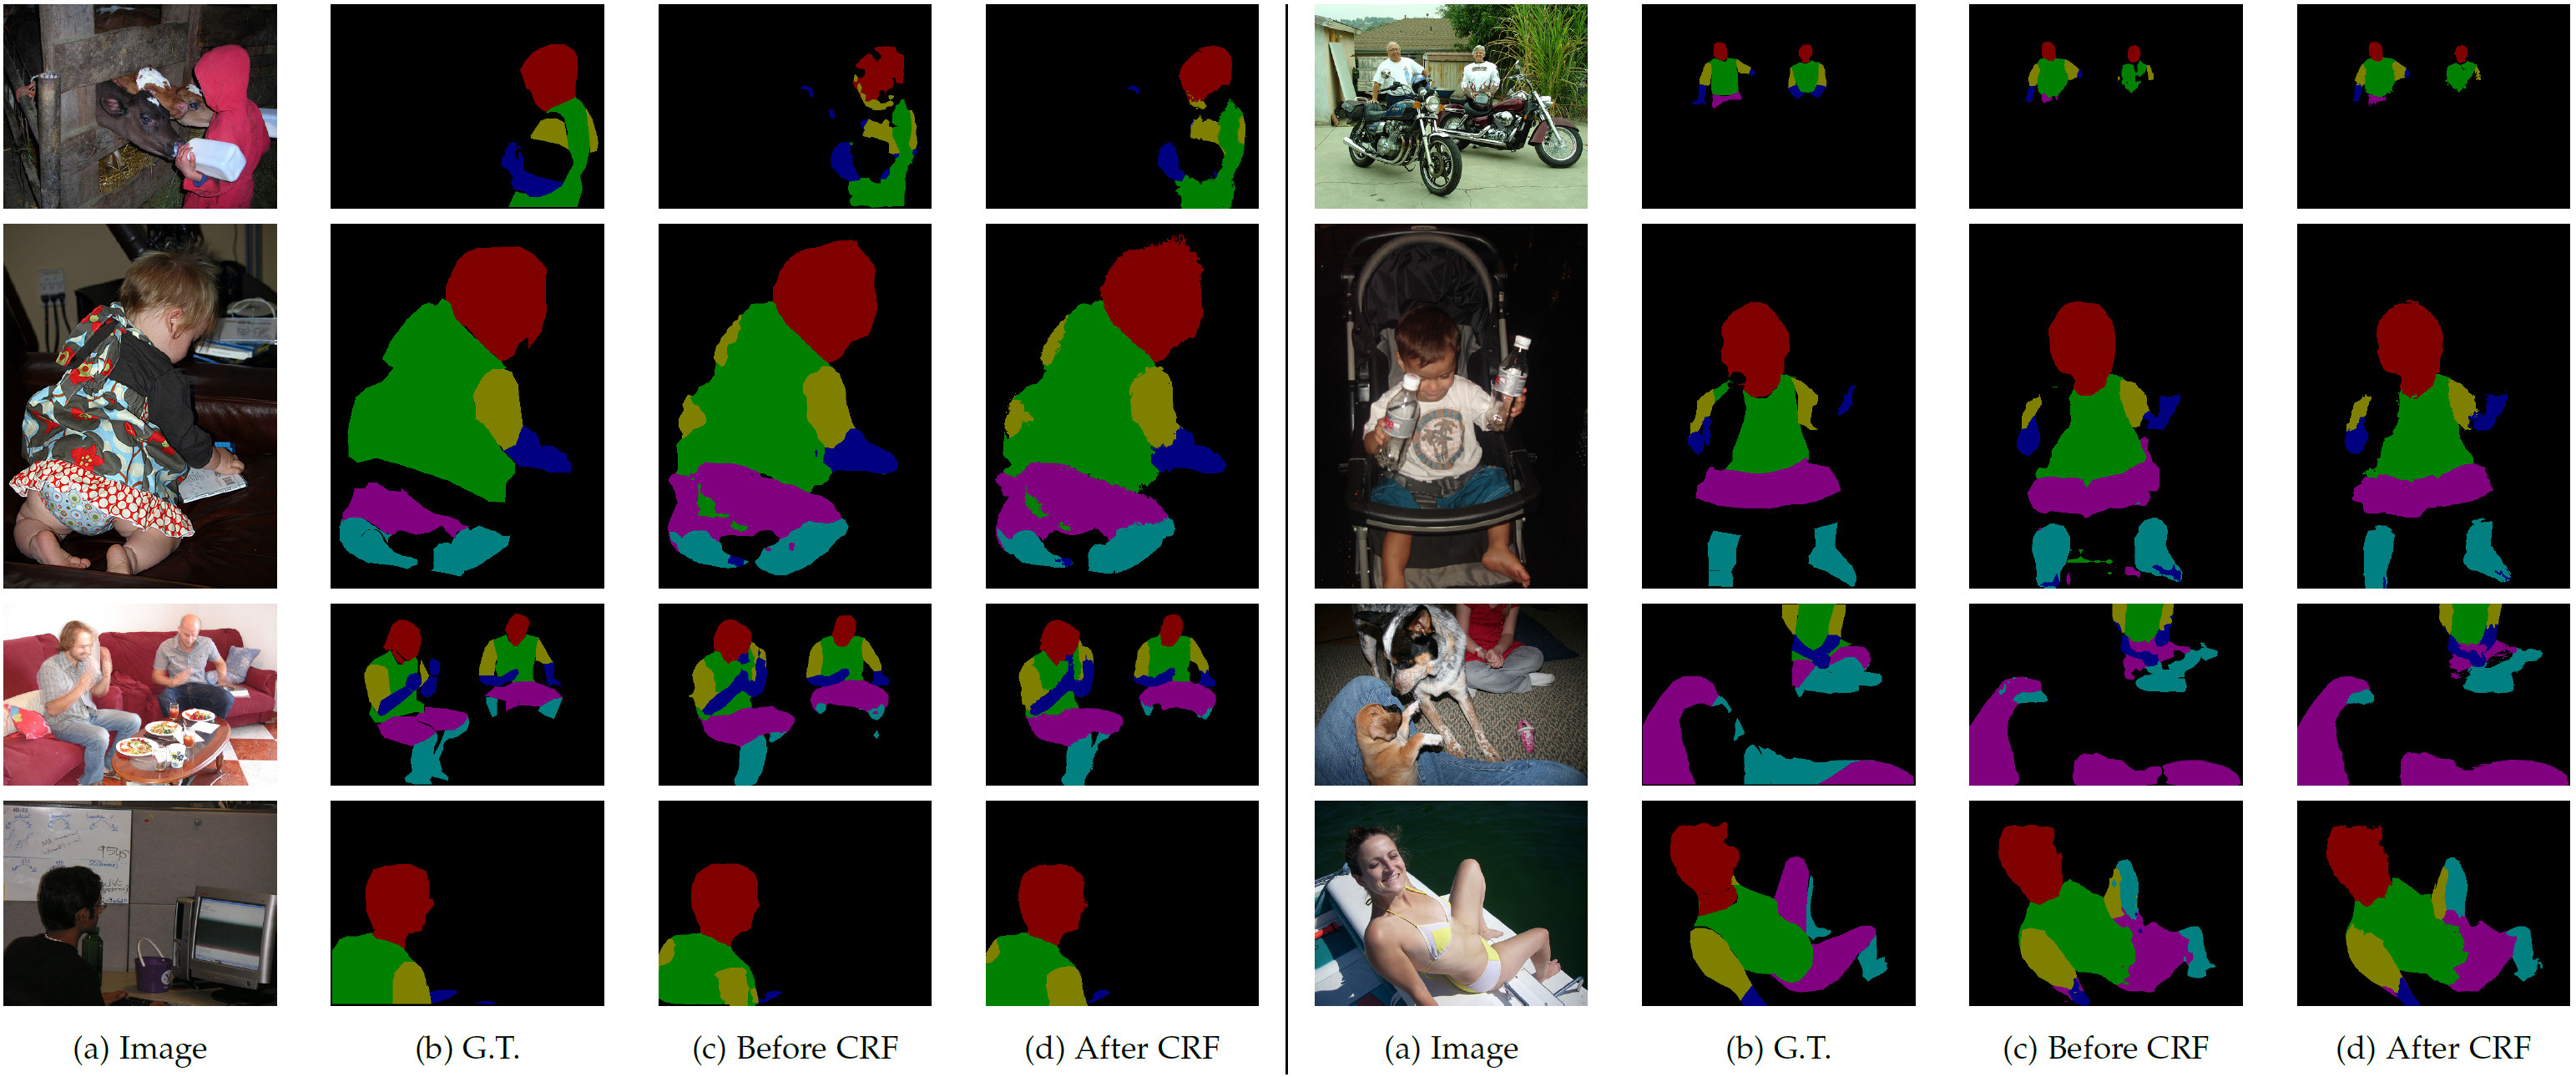
\includegraphics[width=1.\linewidth]{fig/voc10_part/results.jpg} \\
  \end{tabular}
  }
  \caption{PASCAL-Person-Part 结果。原图,真实边界,CRF前后 DeepLab 的运算结果。}
  \label{fig:voc10_part_val_results}
\end{figure*}

\begin{table}[!t]
  \centering
  \addtolength{\tabcolsep}{-3pt}
  \scalebox{0.85}{
    \begin{tabular} {l  c c c c c c | c}
      \toprule[0.2 em]
      {\bf Method} & {\bf MSC} & {\bf COCO} & {\bf Aug} & {\bf LFOV} & {\bf ASPP} & {\bf CRF} & {\bf mIOU} \\
      \toprule[0.2 em]
      \multicolumn{7}{l}{\it ResNet-101} & \\
      DeepLab      & & & & & & & 58.90 \\
      DeepLab      & \checkmark & & \checkmark & & & & 63.10 \\
      DeepLab      & \checkmark & \checkmark & \checkmark & & & & 64.40 \\
      DeepLab      & \checkmark & \checkmark & \checkmark & & & \checkmark & 64.94 \\
      \midrule
      DeepLab      & \checkmark & \checkmark & \checkmark & \checkmark & & & 62.18 \\
      DeepLab      & \checkmark & \checkmark & \checkmark & & \checkmark & & 62.76 \\
      \midrule \midrule
      Attention \cite{chen2015attention} & & & & & & & 56.39 \\
      HAZN \cite{xia2015zoom} & & & & & &  & 57.54 \\
      LG-LSTM \cite{liang2015semantic} & & & & & &  & 57.97 \\
      Graph LSTM \cite{liang2016semantic} & & & & & &  & 60.16 \\
      \bottomrule[0.1 em]
    \end{tabular}
  }
  \caption{与 PASCAL-Person-Part 数据集上其它优质算法的比较。}
  \label{tab:pascal_person_part}
\end{table}

\textbf{数据集:} 我们通过使用额外的 PASCAL VOC 2010 标注 \cite{chen_cvpr14} 进一步进行语义部分分割 \cite{wang2014semantic, wang2015joint}。我们专注于数据集的\textit{人像}部分,其中包含更多的训练数据以及对象比例和人体姿势的大变化。具体来说,数据集包含每个人的详细部分注释,例如眼睛,鼻子。我们将注释合并为头部,躯干,上/下臂和上/下腿,从而产生六个人的部分类和一个背景类。我们仅使用包含人像的图像进行训练(1716张)和验证(1817张)。

\textbf{评估:} \tabref{tab:pascal_person_part} 展示了 DeepLab 在 PASCAL-Person-Part 上的人体部分分割结果。\cite{chen2015attention} 已经针对此数据集进行了实验,重新使用了基于 VGG-16 的 DeepLab,达到了 $56.39\%$ (多尺度输入)。因此,在本部分中,我们主要关注 基于 ResNet-101 的结果。仅使用 ResNet-101 时,DeepLab 达到了 $58.9\%$ 的性能,明显优于DeepLab-LargeFOV(VGG-16)和DeepLab-Attention(VGG-16网络),分别高了 $7\%$ 和 $2.5\%$。通过最大池化结合多尺度输入和融合进一步将性能提高到 $63.1\%$。此外,在MS-COCO上预训练模型产生了另外 $1.3%$ 的改进。但是,在此数据集上采用LargeFOV 或 ASPP时,我们没有观察到任何改进。使用全连接的CRF进行后期处理后,我们的最终输出大大优于同期工作 \cite{liang2016semantic} $4.78\%$。

\textbf{定性结果:} 如 \figref{fig:voc10_part_val_results} 所示,我们对验证集上的结果进行了可视化展示。

\subsection{Cityscapes}
\label{exp:cityscapes}

\begin{figure*}[!t]
  \centering
  \scalebox{1} {
  \begin{tabular}{c}
    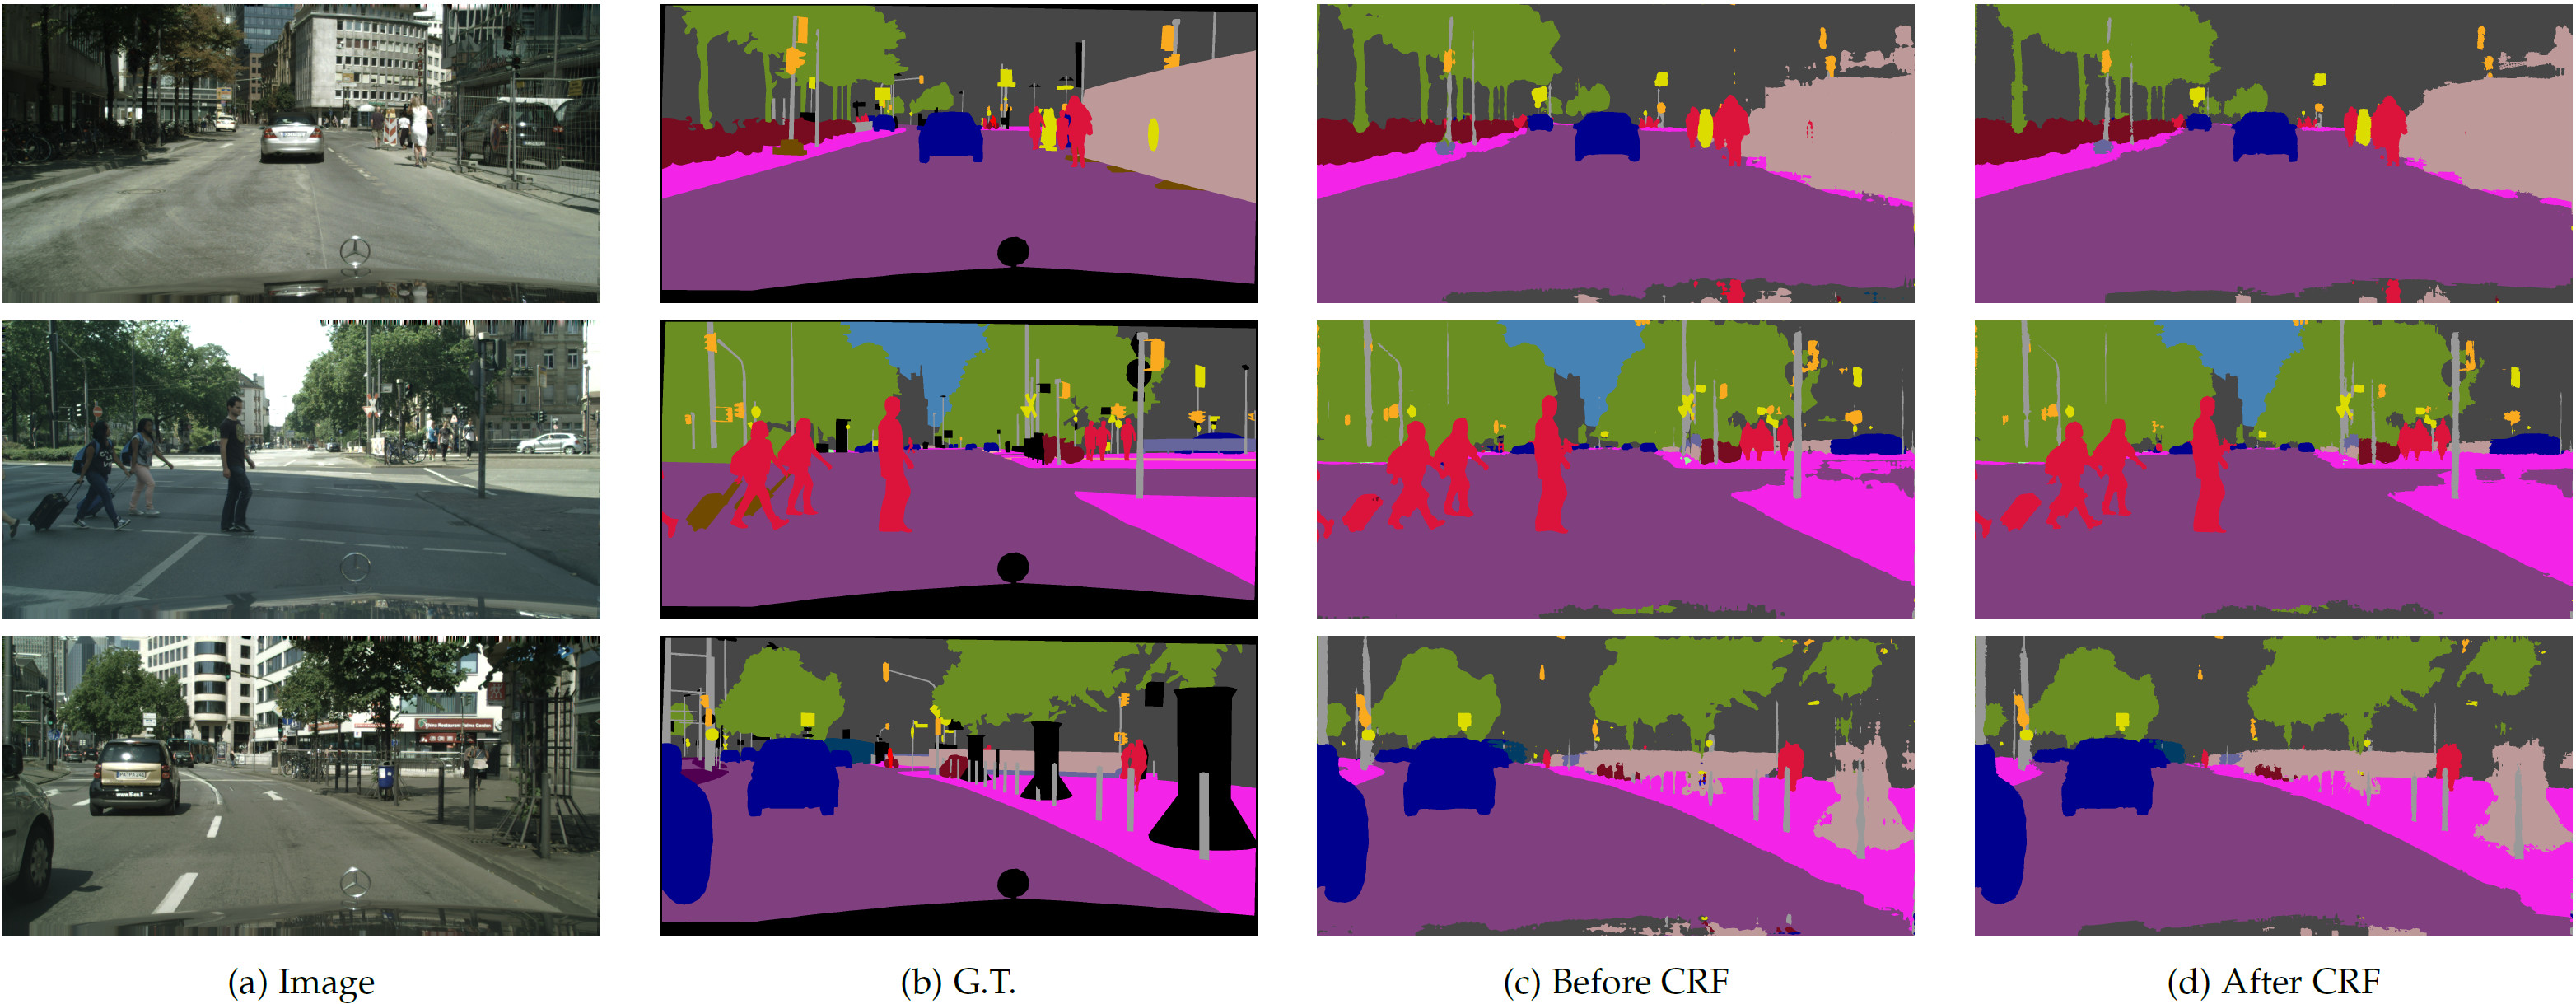
\includegraphics[width=0.9\linewidth]{fig/cityscapes/results.jpg} \\
  \end{tabular}
  }
  \caption{Cityscapes 结果。原图,真实边界,CRF前后 DeepLab 的运算结果。}
  \label{fig:cityscapes_val_results}
\end{figure*}


\begin{table}[!t]
  \centering
  \addtolength{\tabcolsep}{2.5pt}
  \begin{tabular}{l | c}
    \toprule[0.2 em]
    {\bf Method} & {\bf mIOU} \\
    \toprule[0.2 em]
    \multicolumn{2}{l}{\it pre-release version of dataset} \\
    Adelaide\_Context \cite{lin2015efficient} & 66.4 \\
    FCN-8s \cite{long2014fully} & 65.3 \\
    \midrule
    DeepLab-CRF-LargeFOV-StrongWeak \cite{papandreou2015weakly} & 64.8 \\
    DeepLab-CRF-LargeFOV \cite{chen2014semantic} & 63.1 \\
    \midrule
    CRF-RNN \cite{zheng2015conditional} & 62.5 \\
    DPN \cite{liu2015semantic} & 59.1 \\
    Segnet basic \cite{badrinarayanan2015segnet} & 57.0 \\
    Segnet extended \cite{badrinarayanan2015segnet} & 56.1 \\
    \midrule \midrule
    \multicolumn{2}{l}{\it official version} \\
    Adelaide\_Context \cite{lin2015efficient} & 71.6 \\
    Dilation10 \cite{yu2015multi} & 67.1 \\
    DPN \cite{liu2015semantic} & 66.8  \\
    Pixel-level Encoding \cite{uhrig2016pixel} & 64.3 \\
    \midrule
    DeepLab-CRF (ResNet-101) & 70.4 \\
    \bottomrule[0.1 em]
  \end{tabular}
  \caption{与 Cityscapes 数据集上其它优质算法的比较。}
  \label{tab:cityscapes_test}
\end{table}

\begin{table}[!t]
  \centering
  \addtolength{\tabcolsep}{2pt}
  \begin{tabular}{c c c c c | c}
    \toprule[0.2 em]
    {\bf Full} & {\bf Aug} & {\bf LargeFOV} & {\bf ASPP} & {\bf CRF} & {\bf mIOU} \\
    \toprule[0.2 em]
    \multicolumn{5}{l}{\it VGG-16} & \\
    & & \checkmark & & & 62.97 \\
    & & \checkmark & & \checkmark & 64.18 \\
    \checkmark & & \checkmark & & & 64.89 \\
    \checkmark & & \checkmark & & \checkmark & 65.94 \\
    \midrule
    \multicolumn{5}{l}{\it ResNet-101} & \\
    \checkmark & & & & & 66.6 \\
    \checkmark & & \checkmark & & & 69.2 \\
    \checkmark & &  & \checkmark & & 70.4 \\
    \checkmark & \checkmark & & \checkmark & & 71.0 \\
    \checkmark & \checkmark & & \checkmark & \checkmark & 71.4 \\
    \midrule
    \bottomrule[0.1 em]
  \end{tabular}
  \caption{Cityscapes 验证集上的结果。 {\bf Full}: 使用原图分辨率进行训练。}
  \label{tab:cityscapes_val_resnet}
\end{table}

\textbf{数据集:} Cityscapes \cite{Cordts2016Cityscapes} 是最近发布的大型数据集,其中包含来自50个不同城市的街景中收集的5000张图像的高质量像素级标注。根据评估协议 \cite{Cordts2016Cityscapes},19个语义标签(属于7个超类:地面,建筑,对象,自然,天空,人类和车辆)用于评估(不考虑空白标签)。训练、验证和测试集分别包含$2,975$、$500$和$1,525$ 张图像。


\textbf{在预发布测试集上的结果:} 我们参与了 Cityscapes 数据集预发布的基准测试。如 \tabref{tab:cityscapes_test} 所示,我们的模型获得第三名,表现为 $63.1\%$ 和 $64.8\%$(添加训练了额外粗标注图像)。

\textbf{验证集结果:}
在初始发布之后,我们进一步探索了 \tabref{tab:cityscapes_val_resnet} 中的其他验证集。Cityscapes 的图片分辨率为 \by{2048}{1024},因此训练具有有限 GPU内存 的更深层网络成为一个具有挑战性的问题。在对数据集的预发布进行基准测试期间,我们将图像下采样率设为2。然而,我们发现以原始分辨率处理图像是有益的。使用相同的训练方法,使用原始分辨率的图像分别在 CRF前后 带来了 $1.9\%$ 和 $1.8\%$ 的性能改进。为了使用高分辨率图像对此数据集进行推断,我们将每个图像拆分为若干重叠区域,类似于 \cite{Cordts2016Cityscapes}。我们还用 ResNet-101 取代了 VGG-16。由于手头的 GPU内存 有限,我们没有使用多尺度输入。然而我们探索了(1)更深的网络结构(\ie, ResNet-101)(2)数据增益(3)使用 LargeFOV 或者 ASPP(4)用 CRF 作为后续处理手段。我们发现单独使用ResNet-101比使用VGG-16更好。使用LargeFOV可带来$2.6\%$的性能提升,使用ASPP可进一步提高$1.2\%$。采用数据增益和CRF作为后处理分别带来另外$0.6\%$和$0.4\%$提升。

\textbf{当前测试集结果:} 我们将最优的模型上传到了官方评估服务器上,获得了 $70.4\%$ 的 IOU。而这个模型是仅在官方训练集上训练的。

\textbf{定性结果:} 在 \figref{fig:cityscapes_val_results} 中,我们对验证集结果进行了可视化处理。

\subsection{失真情况}

我们进一步定性分析了 PASCAL VOC 2012 验证集中我们最佳模型的一些失真情况。如 \figref{fig:failure_modes} 所示,我们提出的模型无法捕捉到物体的微妙边界,例如自行车和椅子。因为一元项不够充分,CRF后期处理甚至无法恢复细节。我们假设 \cite{badrinarayanan2015segnet, ronneberger2015u} 的编码器 - 解码器结构可以通过利用解码器路径中的高分辨率特征图来解决该问题。 如何有效地整合该方法是我们未来的研究内容。

\begin{figure}[!t]
\centering
\resizebox{\columnwidth}{!}{
  \begin{tabular} {c c c c}
    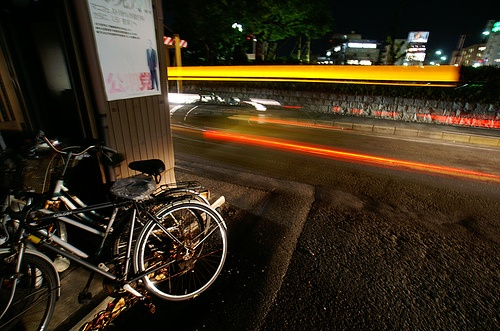
\includegraphics[width=0.24\linewidth]{fig/failure_mode/voc12/resnet101_noup_pool3_coco_22/img/2007_000572.jpg} &
    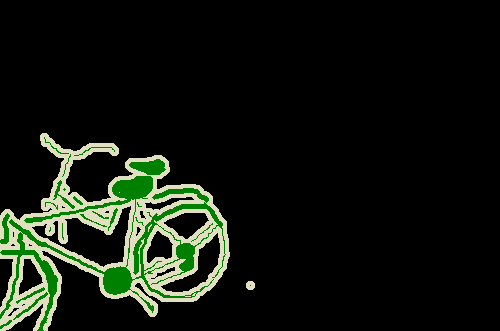
\includegraphics[width=0.24\linewidth]{fig/failure_mode/voc12/resnet101_noup_pool3_coco_22/gt/2007_000572.png} &
    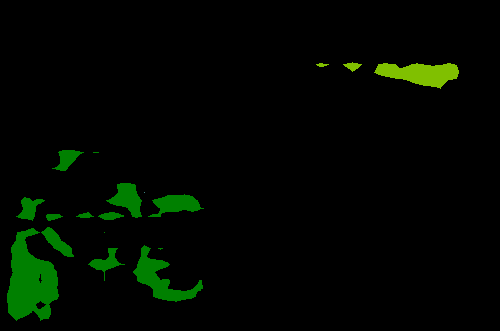
\includegraphics[width=0.24\linewidth]{fig/failure_mode/voc12/resnet101_noup_pool3_coco_22/before_crf/2007_000572.png} &
    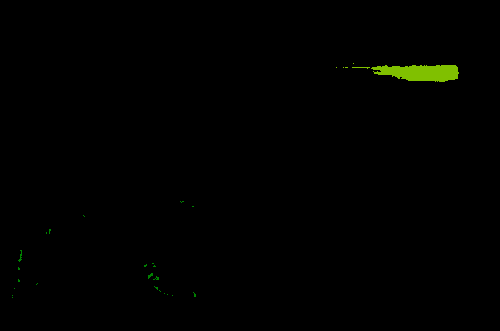
\includegraphics[width=0.24\linewidth]{fig/failure_mode/voc12/resnet101_noup_pool3_coco_22/after_crf/2007_000572.png} \\
    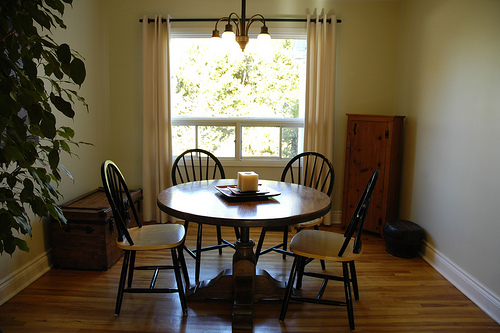
\includegraphics[width=0.24\linewidth]{fig/failure_mode/voc12/resnet101_noup_pool3_coco_22/img/2009_002487.jpg} &
    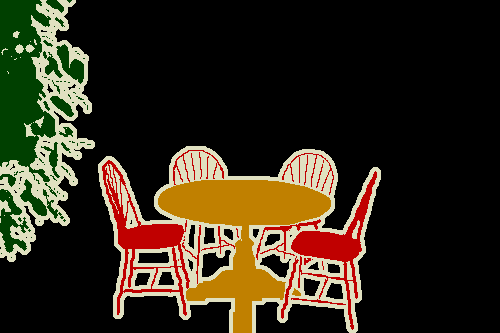
\includegraphics[width=0.24\linewidth]{fig/failure_mode/voc12/resnet101_noup_pool3_coco_22/gt/2009_002487.png} &
    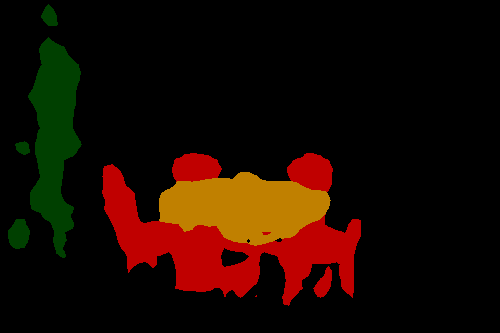
\includegraphics[width=0.24\linewidth]{fig/failure_mode/voc12/resnet101_noup_pool3_coco_22/before_crf/2009_002487.png} &
    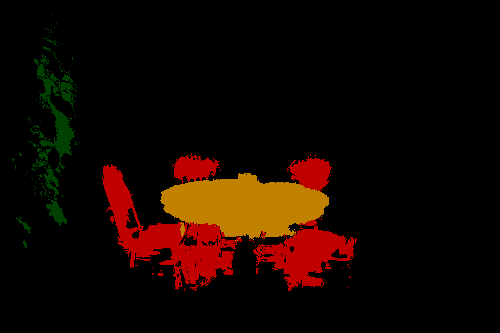
\includegraphics[width=0.24\linewidth]{fig/failure_mode/voc12/resnet101_noup_pool3_coco_22/after_crf/2009_002487.png} \\
                    {\scriptsize (a) Image} &
                    {\scriptsize (b) G.T.} &
                    {\scriptsize (c) Before CRF} &
                    {\scriptsize (d) After CRF} \\
  \end{tabular}

}
  \caption{失真情况。原图,真实边界,CRF前后 DeepLab 的运算结果。}  
  \label{fig:failure_modes}
\end{figure}
